\documentclass[UTF8]{ctexart}

\usepackage{subfiles}  

%下面的语句, 引入你的头部设置文件
\usepackage{C:/phpStorm_proj/02_myself_ID_EGO/+100_latex_all_math_sel/myPreamble} 
%必须是绝对路径,才能让各个tex在单独编译时使用到

\title{积分}


%---------------------------------


\begin{document}
	\tableofcontents % 生成目录
	\date{} % 若不写这句, 则默认也会渲染出日期, 所以我们要手动赋空值
	\maketitle  %这行代码, 让你前面的 title, author, date生效
	
	\part{定积分 definite integral}
	
	
	\section{``定积分"的定义}
	
	1. 曲线函数f(x), 在x轴上有界, 比如端点是[a,b].
	
	2. 然后, 我们在[a,b]这段区间上, 任意插入n个分点, 分成n个小区间. 它们不要求等分. 每个小区间的长度就是 $ \Delta x_1, \Delta x_2,..., \Delta x_n$.
	
	3. 在每个Δ小区间上, 任取一点 $ \xi_i$. 这点的函数值(即y轴上的高度), 就是 $ y=f(\xi_i)$.
	
	4. 这样, 我们就能得到每一个Δ小区间, 所在的``长方形细条的面积"了, 即 $= \text{宽} \Delta x_i \cdot \text{高}f(\xi_i)$
	
	5. 把所有这些Δ小区间的``长方形细条面积", 全加起来, 就是该曲线到x轴间的面积的近似值. $ = \sum_{i=1}^n \Delta x_i\cdot f(\xi _i) $
	
	6. 我们令其中 x轴宽度最大的那个Δx小区间 (假设起名为λ, 即$ \lambda =\max \left\{ \varDelta x_1,...,\varDelta x_n \right\} $), 我们让这个λ, 极限趋向于0. 这样, 既然最大的 Δx小区间 都趋近于0了, 其他比它更小的 Δx小区间, 就都统统被约束, 也都趋向于0了. 这样, 它们的``长方形细条的面积之和", 就能精确的等于``函数曲线到x轴之间的面积"了, 而不仅仅是``近似"了. \\
	
	即: 
	$	\lim_{x\rightarrow 0}\sum_{i=1}^n{\underset{\text{高}}{\underbrace{f\left( \xi _i \right) }}\cdot \underset{\text{宽}}{\underbrace{\varDelta x_i}}=\underset{\text{定积分}}{\underbrace{\int_a^b{f\left( x \right)}dx}}}	$ \\
	
	各部分的名字是:
	$
	\int_{\text{下限}a}^{\text{上限}b}{\underset{\text{被积表达式}}{\underbrace{\underset{\text{被积函数}}{\underbrace{f\left( x \right) }}\ d\underset{\text{积分变量}}{\underbrace{\left( x \right) }}}}}
	$
	
	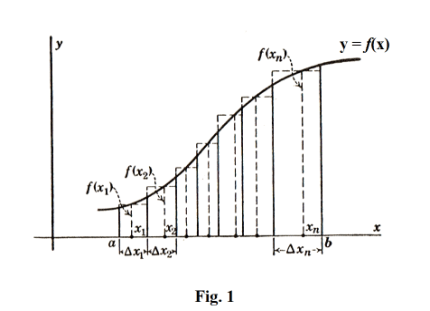
\includegraphics[width=0.5\textwidth]{/0060.png}
	
	
	
	
	
	\section{定积分的性质}
	
	\subsection{若 b=a, 则 $ \int_a^a f(x) = 0$}
	
	\subsection{$ \int_a^b f(x) = -  \int_b^a f(x)$  ← 交换上下限, 定积分的值要变号}
	
	\subsection{$\int_a^b (\alpha \cdot f(x) + \beta \cdot g(x)) dx = \alpha \int_a^b  f(x) dx + \beta \int_a^b  g(x) dx$ ← 即, 积分可以拆开, 常数可以提到外面去}
	
	\subsection{ 若 $ a < c < b$, 则 $ \int_a^b f(x) dx = \int_a^c f(x) dx + \int_c^b f(x) dx $ ← 其实就是原先的一步走, 分成两步走而已.}
	
	
	\subsection{ 若 $ a < b < c$, 则: $ \int_a^b f(x) dx = \int_a^c f(x) dx - \int_c^b f(x) dx$} 
	
	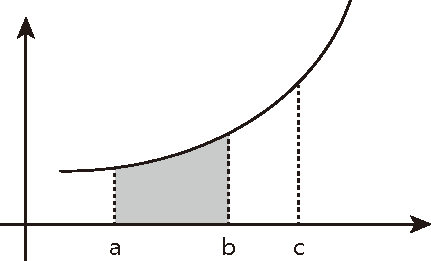
\includegraphics[width=0.4\textwidth]{/0061.pdf}
	
	
	
	\subsection{若 f(x) 恒等于1, 即该函数是条``水平直线", 它与x轴之间就形成一个矩形了. 则 $ \int_a^b 1 dx = \text{高}1 \cdot \text{宽}(b-a) = b-a$}
	
	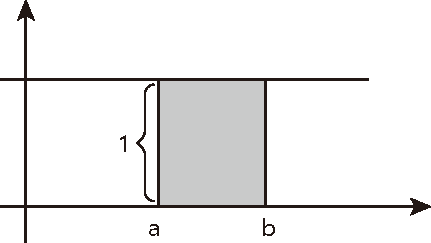
\includegraphics[width=0.4\textwidth]{/0062.pdf}	
	
	
	\subsection{$\int_a^b k dx = k  \int_a^b 1 dx =  k(b-a) $ ← k 是常数, 可以提到积分外面}
	
	\subsection{若 $ f(x) >= 0$, 即``函数曲线"都在x轴上方.  则$ \int_a^b f(x) dx >= 0$}
	
	\subsection{若$ f(x) <= 0$, 即``函数曲线"都在x轴下方.  则  $\int_a^b f(x) dx <= 0$}
	
	\subsection{若 $ f(x) <= g(x)$, 则 $ \int_a^b f(x) dx  <=  \int_a^b g(x) dx$ }
	
	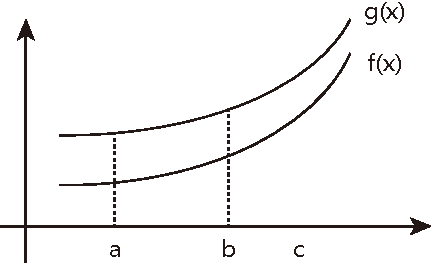
\includegraphics[width=0.4\textwidth]{/0063.pdf}
	
	
	\subsection{$|\int_a^b f(x) dx | <= \int_a^b |f(x)| dx$} 
	
	因为``函数曲线"的定积分(面积), 在x轴上方是正面积的, 在x轴下方是负面积的, 如果一个曲线既有正y值的部分, 又有负y值的部分, 那它的总面积, 肯定会有"正负相互抵消掉"的一部分.
	
	而先把``函数曲线"取绝对值, 它的y值就都在x轴上方了, 面积就不存在负数的一块, 就不会抵消掉总面积. \\
	
	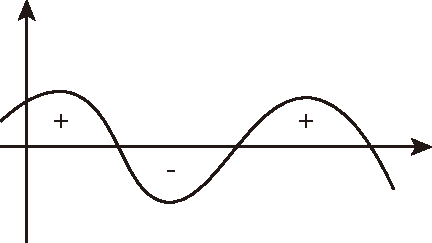
\includegraphics[width=0.4\textwidth]{/0064.pdf}	
	
	
	
	\subsection{一个曲线, 在[a,b]区间上, 若 m是它的最小y值高度, M是它的最大y值高度, 则有: $ m(b-a) \leq \int_a^b f(x) dx  \leq M(b-a)$}
	
	如下图, ``高m" 乘以 ``宽(b-a)", 就是 abm 这个小矩形的面积.
	
	`高M" 乘以 `宽(b-a)", 就是 abM 这个大矩形的面积.
	
	曲线mM 的定积分, 这个面积大小, 肯定是夹在上面两个矩形的面积之间的. \\
	
	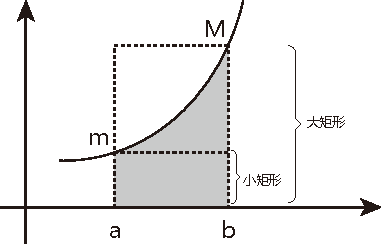
\includegraphics[width=0.4\textwidth]{/0065.pdf}
	
	使用该方法, 就可以让我们来对曲线的定积分值, 进行估计.
	
	
	
	\subsection{定积分``中值定理" : \\
		如果 f(x) 是连续的, $ \exists \xi  \in [a,b], \text{则必然有}\int_a^b{f(x)dx=f(\xi)(b-a)}$}
	
	定积分中值定理 Mean value theorems for definite integrals 的意思就是说: 在函数曲线的 [a,b]区间上, 一定能找到一个点 $\xi$, 该$\xi$点的 y值高度(即 f($\xi$)), 乘上 ``b-a 这个宽度", 所形成的的矩形面积, 能恰好等于 函数曲线的定积分值.  你找吧, 一定能找到这个点$\xi$ 存在. \\
	
	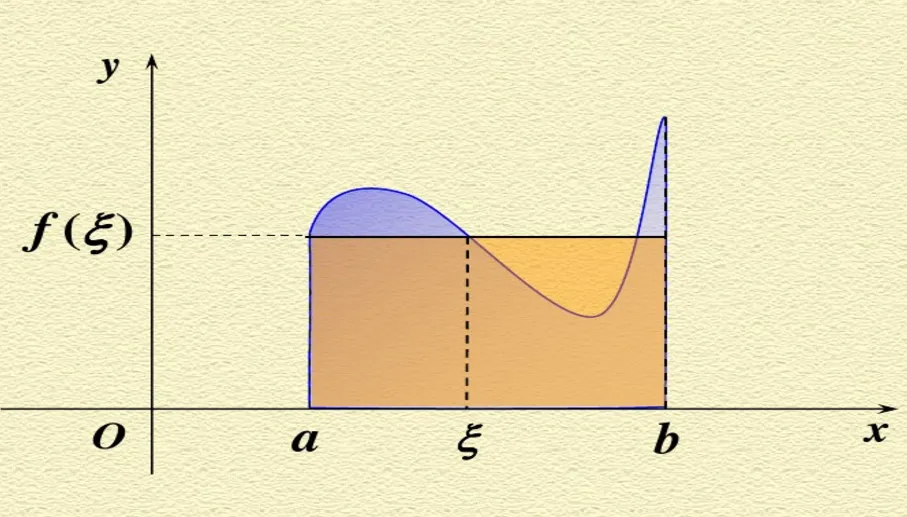
\includegraphics[width=0.5\textwidth]{/0066.png}
	
	
	~\\
	\hrule
	~\\
	
	\part{求定积分的方法}
	
	
	\section{定积分的``分部积分法": $\int_a^b{\text{前}\cdot d(\text{后})}=\left( \text{前}\cdot \text{后} \right) \mid_{a}^{b}-\int_a^b{\text{后}}\ d(\text{前})$}
	
	比较一下: 
	
	``不定积分"的``分部积分法"公式是: $\boxed{\int_{}^{}{\text{前}\cdot d(\text{后})}=\text{前}\cdot \text{后}-\int_{}^{}{\text{后}}\ d(\text{前})}	$
	
	`定积分"的``分部积分法"公式是: $\boxed{\int_a^b{\text{前}\cdot d(\text{后})}=\left( \text{前}\cdot \text{后} \right) \mid_{a}^{b}-\int_a^b{\text{后}}\ d(\text{前})}	$ \\
	
	为什么要用``分部积分法", 来把 d(后) 变成d(前)? 不还是要求某个数的微分么? 其实, 你这样做的目的, 是需要先满足这个前提的: 即: 
	当 ``$\int_{}^{}{\text{后\ }d\left( \text{前} \right)}$" 比 ``$\int_{}^{}{\text{前\ }d\left( \text{后} \right)}$" 更容易算时, 你可以用``分部积分法"来交换微分的顺序.
	
	注意: 在反复使用分部积分法的过程中, 不要对调两个函数地位, 否则不仅不会产生循环现象, 反而会一来一往, 恢复原状, 毫无所得.
	
	
	
	
	
	
	
	
	
	\begin{myEnvSample}
	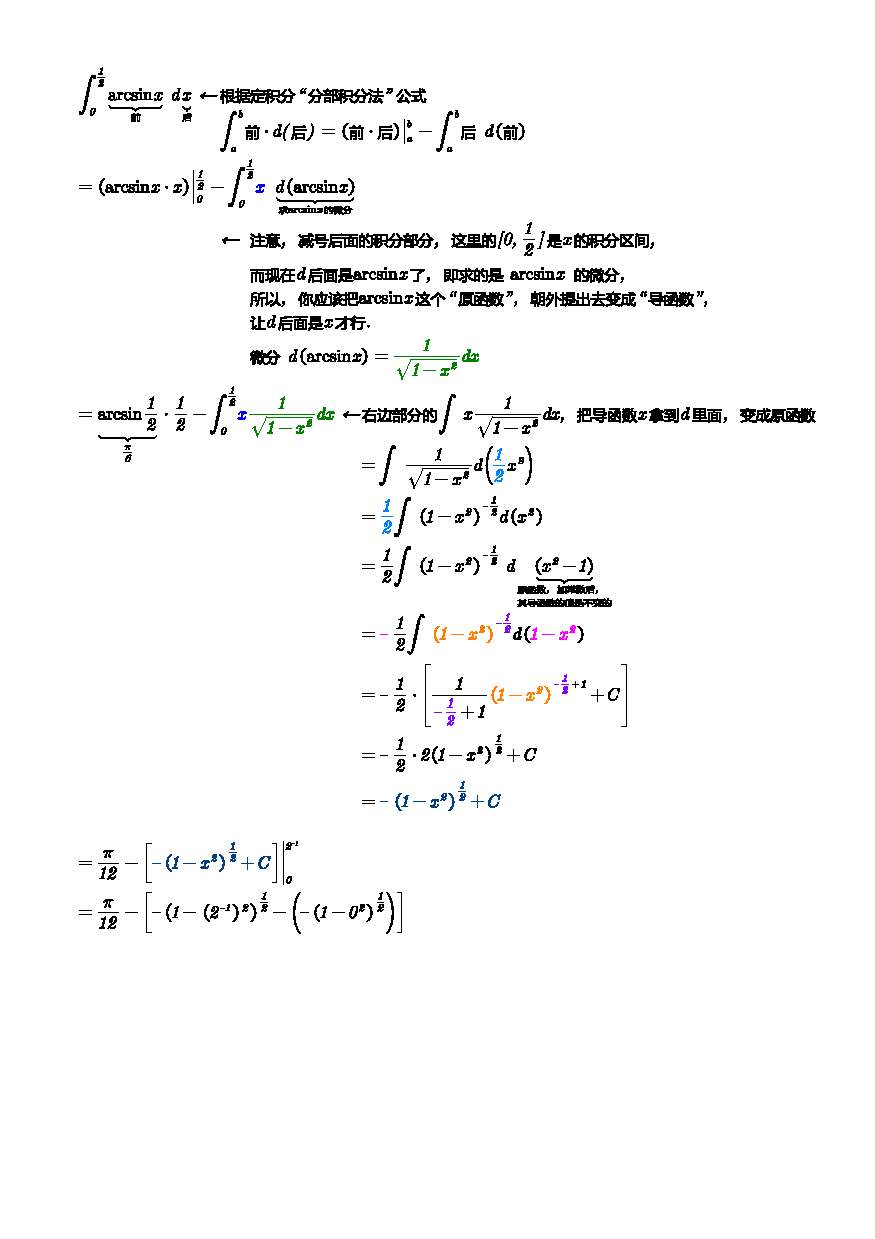
\includegraphics[width=1\textwidth]{/0067.pdf}
	\end{myEnvSample}
	

\begin{myEnvSample}
	$\int_0^1{e^{\sqrt{x}}}\ dx$ 
	
	我们用换元法, 令$\sqrt{x}=t$, 则$x=t^2$. 于是, $dx=\underset{\text{求微分}}{\underbrace{d\left( t^2 \right) }}=\left( t^2 \right) 'dt=2t\ dt$
	
	→ 原上限是 x=1, 换成t来表示上限, 就是 $x=t^2=1$, 即 t=1, 这个就是换元成t后的 t的新上限.
	
	→ 原下限是x=0, 换成t来表示上限, 就是 $x=t^2=0$, 即 t=0. 这个是t的下限.
	
	所以原式就变换成了: 
	\begin{align*}
		&=\int_0^1{e^t}\ 2t\ dt=2\int_0^1{e^t}\ t\ dt\ \gets \text{把导函数}t,\text{拿到微分}d\text{后面,\ 变成原函数}.\\
	&=2\int_0^1{\underset{\text{前}}{\underbrace{t}}}\ d\underset{\text{后}}{\underbrace{\left( e^t \right) }}\ \gets \text{使用定积分的``分部积分法"}\\
	&=2\left[ t\cdot e^t\mid_{0}^{1}-\int_0^1{e^t\ d\left( t \right)} \right] =2\left[ 1\cdot e-e^t\mid_{0}^{1} \right] =2\left[ e-\left( e^1-e^0 \right) \right] =2
	\end{align*}

%		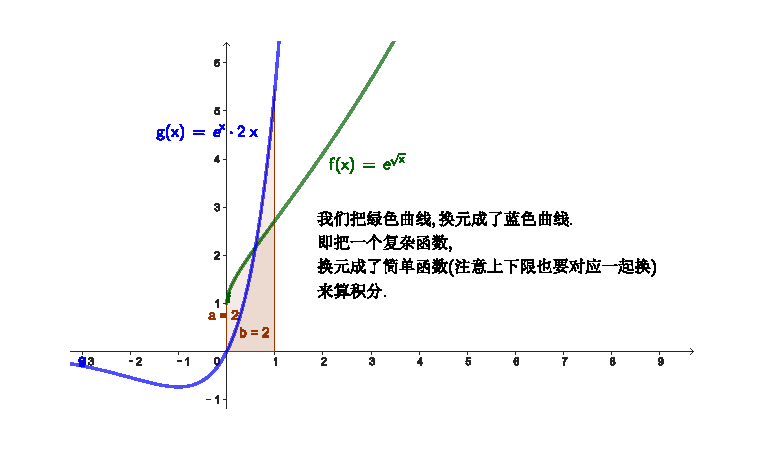
\includegraphics[width=0.4\textwidth]{/0068.pdf}

\end{myEnvSample}
	

	
	
	
\end{document}


